\documentclass[11pt,a4paper]{article}

\usepackage[utf8]{inputenc}
\usepackage[T1]{fontenc}
\usepackage[french]{babel}
\usepackage{graphicx}
\usepackage{amsmath}
\usepackage{amssymb}

\title{Analyse des performances des tris}
\author{NIDDAM Benjamin}
\date{28 Novembre 2020}

\begin{document}
\maketitle
\begin{center}
    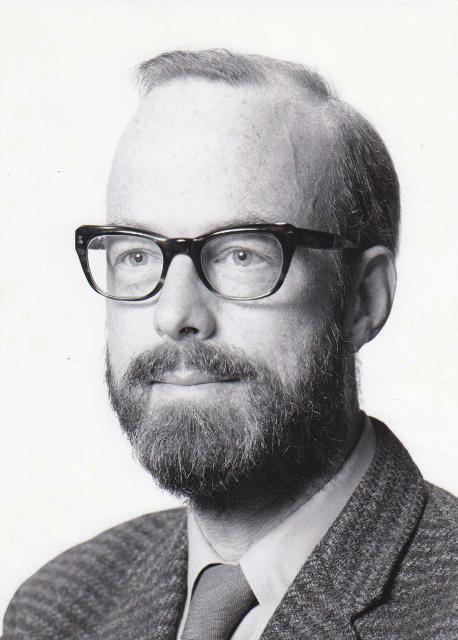
\includegraphics{Images/Tony Hoare.jpg}
    \newline
    \newline
    En 1962, Tony Hoare inventa le tri rapide (Quicksort), qui est généralement considéré comme l'algorithme le plus utilisé dans le monde entier.
\end{center}

\newpage
\tableofcontents
\newpage
\section{Introduction}

\subsection{Définition}

\paragraph{}
Un algorithme de tri est, en informatique ou en mathématiques, un algorithme qui permet d'organiser une collection d'objets
selon une relation d'ordre déterminée.
\newline
La collection à trier est souvent donnée sous forme de tableau, afin de permettre l'accès direct aux différents éléments de la collection,
ou sous forme de liste, ce qui peut se révéler être plus adapté à certains algorithmes et à l'usage de la programmation fonctionnelle.\\

\paragraph{}
Aujourd'hui on retrouve de nombreux algorithmes de tri que l'on peut diviser en 3 grandes catégories:
\begin{itemize}
    \item Les Tris par comparaison
    \item Les Tris utilisant la structure de données
    \item Les Tris externes
\end{itemize}
\vspace{0.5cm}
Les tris par comparaison peuvent encore se diviser en 4 sous catégories en fonction de leur vitesse d'exécution:

\vspace{0.2cm}
\begin{itemize}
    \item Les algorithmes rapides avec une complexité moyenne de $n*\log(n)$
    \item Les algorithmes moyennement rapides (En moyenne O($n^2$), O($n$) dans le meilleur des cas)
    \item Les algorithmes lents avec une complexité de O($n^2$) dans tous les cas
    \item Les algorithmes très lents avec une complexité moyenne moins bonne que O($n^2$)
\end{itemize}

\subsection{Exemples}
\subsubsection{Les Tris par comparaison}
\begin{itemize}
    \item Le tri fusion (dit merge sort)
    \item Le tri rapide (dit quicksort)
    \item Le tri par tas (dit heap sort)
    \item Le tri fusion (dit merge sort)
    \item Le tri par insertion
    \item Le tri à bulle
    \item Le tri par sélection
    \item Le tri stupide
    \item Le tri faire-valoir
\end{itemize}
\newpage
\subsubsection{Les Tris utilisant la structure de données}
\begin{itemize}
    \item Le tri comptage ou tri par dénombrement
    \item Le tri par base
    \item Le tri par paquets
\end{itemize}

\subsubsection{Les Tris externes}
Ces algorithmes sont souvent basés sur une approche assez voisine de celle du tri fusion. Le principe est le suivant :
\vspace{0.2cm}

\begin{itemize}
    \item découpage du volume de données à trier en sous-ensembles de taille inférieur à 0.02 secondes  à la mémoire rapide disponible ;
    \item tri de chaque sous-ensemble en mémoire centrale pour former des "monotonies" (sous-ensembles triés) ;
    \item interclassement des monotonies.
\end{itemize}

\section{Critères de classification}
La classification des algorithmes de tri est très importante, car elle permet de choisir l’algorithme le plus adapté au problème traité,
tout en tenant compte des contraintes imposées par celui-ci. Les principales caractéristiques qui permettent de différencier les algorithmes
de tri, outre leur principe de fonctionnement, sont la complexité temporelle, la complexité spatiale et le caractère stable.

\newpage
\subsection{Complexité algorithmique ou temporelle}
Afin d’évaluer la complexité des différents algorithmes de tri présentés, on comptera le nombre de comparaisons et d’échanges de valeur entre deux
éléments du tableau sans prendre en compte les affectations et comparaisons sur des variables de comptage de boucles.\\
\vspace{0.1cm}

Les méthodes présentées sont de deux types :
\begin{itemize}
    \item des méthodes qui trient les éléments deux à deux, de manière plus ou moins
          efficace, mais qui nécessitent toujours de comparer chacun des N éléments avec
          chacun des $N-1$ autres éléments, donc le nombre de comparaisons sera de l’ordre
          de $n^2$ — on note cet ordre de grandeur $\displaystyle{O(n^2)}$.
          \vspace{0.1cm}

          Par exemple, pour $n=1000$, $n^2=10^6$, pour $n=10^6$, $n^2=10^{12}$.
          \vspace{0.2cm}

          Les algorithmes de ce type sont :
          \begin{itemize}
              \item une méthode de tri élémentaire, le tri par sélection ;
              \item et sa variante, le tri par propagation ou tri bulle ;
              \item une méthode qui s’apparente à celle utilisée pour trier ses cartes dans un jeu, le tri par insertion ;
          \end{itemize}
          \vspace{0.2cm}

    \item des des méthodes qui sont plus rapides, car elles trient des sous-ensembles de ces N éléments puis regroupent les
          éléments triés, elles illustrent le principe « diviser pour régner ». Le nombre de comparaisons est alors de l’ordre de
          $n*\log(n)$.
          \vspace{0.1cm}

          Par exemple, pour $n=1000$, $n*\log(n)=10000$ environ, pour ${n=10^6}$, $n*\log(n)=20*10^6$ environ.
          \vspace{0.2cm}

          Les algorithmes de ce type sont :
          \begin{itemize}

              \item le fameux tri rapide ou Quicksort ;
              \item et enfin, le tri par fusion.
          \end{itemize}
          \vspace{0.1cm}

          Cette liste n’est évidemment pas exhaustive. Il existe des méthodes particulièrement adaptées à certains types de données spécifiques.
          Le tri par base (dit radix sort) en est un exemple.

          \vspace{0.5cm}

          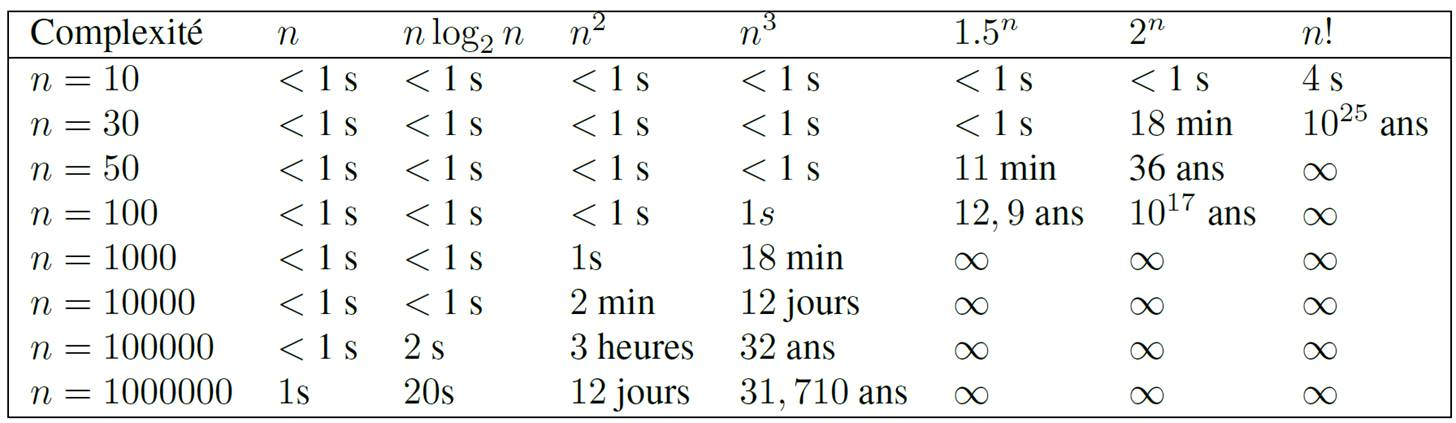
\includegraphics[scale = 0.5]{Images/O(n).jpg}
          \underline {FIGURE 1 - Temps d'éxécution en fonction de la compléxité et du nombre d'éléments}


\end{itemize}

\subsection{Complexité spatiale}
De la même façon qu’on définit la complexité temporelle d’un algorithme pour évaluer ses performances en
temps de calcul, on peut définir sa complexité spatiale pour évaluer sa consommation en espace mémoire. Le
principe est le même sauf qu’ici on cherche à évaluer l’ordre de grandeur du volume en mémoire utilisée : il
ne s’agit pas d’évaluer précisément combien d’octets sont consommés par un algorithme mais de préciser son
taux de croissance en fonction de la taille n de l’entrée. Cependant, on notera que la complexité spatiale est
bien moins que la complexité temporelle un frein à l’utilisation d’un algorithme : on dispose aujourd’hui le
plus souvent d’une quantité pléthorique de mémoire vive, ce qui rend moins importante la détermination de la
complexité spatiale.\\
Cette derniere s'exprime de la même facon que la complexité temporelle, sous la forme de $\displaystyle{O(fonction)}$.

\subsection{Tri en place}
En algorithmique, la complexité en espace est une mesure de l'espace utilisé par un algorithme, en fonction des caractéristiques de ses entrées.
L'espace compte le nombre maximum de cases mémoire utilisées simultanément pendant un calcul. Par exemple le nombre de symboles qu'il faut
conserver pour pouvoir continuer le calcul. Usuellement l'espace que l'on prend en compte lorsque l'on parle de l'espace nécessaire pour des
entrées ayant des propriétés données est l'espace nécessaire le plus grand parmi ces entrées ; on parle de complexité en espace dans le pire cas.
Les études de complexité portent dans la majorité des cas sur le comportement asymptotique, lorsque les grandeurs des entrées qui influent sur la
complexité spatiale tendent vers l'infini, et on utilise couramment les notations grand O de Landau.

\subsection{Tri stable}
Un algorithme de tri stable est un algorithme de tri conservant l'ordre initial de deux éléments égaux. Pour définir cette notion, il est nécessaire
que la collection à trier soit ordonnée d'une certaine manière (ce qui est souvent le cas pour beaucoup de structures de données, par exemple pour
les listes ou les tableaux). Les algorithmes de tri instables peuvent être retravaillés spécifiquement afin de les rendre stables, cependant cela peut
être aux dépends de la rapidité et/ou peut nécessiter un espace mémoire supplémentaire. Parmi les algorithmes listés plus bas, les tris stables sont :
\begin{itemize}
    \item le tri à bulles
    \item le tri par insertion
    \item et le tri fusion
\end{itemize}
Les autres algorithmes nécessitent $\displaystyle{O(n)}$ mémoire supplémentaire pour stocker l'ordre initial des éléments.

\subsection{Tri interne et externe}
Un algorithme de tri externe sert à ordonner les éléments d’un fichier stocké partiellement ou entièrement en mémoire externe
(disque). Il existe des algorithmes spécialisés pour trier des fichiers trop grand
pour la mémoire vive : en une telle application, on veut minimiser l’accès à la
mémoire externe. Le tri interne se fait sur un fichier stocké entièrement en
mémoire vive. Le plus souvent, on considère le tri d’un tableau  A$\left[ 0...n-1 \right]$;
parfois, on peut adapter aussi un tel algorithme aux listes chaînées.

\subsection{Tri parallèle}
Certains algorithmes permettent d'exploiter les capacités multitâches de la machine. Notons également que certains algorithmes, notamment ceux qui fonctionnent
par insertion, peuvent être lancés sans connaître l'intégralité des données à trier ; on peut alors trier et produire les données à trier en parallèle.

\section{Présentation des tris}
\subsection{Le tri fusion}
En informatique, le tri fusion est un algorithme de tri par comparaison stable. Sa complexité temporelle pour une entrée de taille n est de l'ordre de
$\displaystyle{n * \log n}$ et sa complexité spaciale est de $\displaystyle{O(1)}$ dans le meilleur cas et de $\displaystyle{O(n)}$ dans le pire,
ce qui est asymptotiquement optimal. Ce tri est basé sur la technique algorithmique diviser pour mieux régner. L'opération principale de
l'algorithme est la fusion, qui consiste à réunir deux listes triées en une seule. L'efficacité de l'algorithme vient du fait que deux listes triées peuvent être
fusionnées en temps linéaire.\\
Le tri fusion se décrit naturellement sur des listes et c'est sur de telles structures qu'il est à la fois le plus simple et le plus rapide. Cependant, il fonctionne
aussi sur des tableaux. La version la plus simple du tri fusion sur les tableaux a une efficacité comparable au tri rapide, mais elle n'opère pas en place : une zone
temporaire de données supplémentaires de taille égale à celle de l'entrée est nécessaire (des versions plus complexes peuvent être effectuées sur place
mais sont moins rapides). Sur les listes, sa complexité est optimale, il se montre très simplement et ne requiert pas de copie en mémoire temporaire.

\newpage

\subsection{Le tri rapide}
En informatique, le tri rapide ou tri pivot (en anglais quicksort) est un algorithme de tri inventé par C.A.R. Hoare en 1962 et fondé sur la méthode de conception
"diviser pour mieux régner". Il est généralement utilisé sur des tableaux, mais peut aussi être adapté aux listes. Dans le cas des tableaux, c'est un tri en place
mais non stable.\\
La complexité moyenne du tri rapide pour $\displaystyle{n}$ éléments est proportionnelle à $\displaystyle{n * \log n}$ et sa complexité spaciale est de $\displaystyle{O(\log n)}$ dans le
meilleur cas et de $\displaystyle{O(n)}$ dans le pire, ce qui est optimal pour un tri par comparaison,
mais la complexité dans le pire des cas est quadratique. Malgré ce désavantage théorique, c'est en pratique un des tris les plus rapides, et donc un des plus utilisés.
Le pire des cas est en effet peu probable lorsque l'algorithme est correctement mis en œuvre et il est possible de s'en prémunir définitivement avec la variante Introsort.

\subsection{Le tri par tas}
En informatique, le tri par tas est un algorithme de tri par comparaisons. Cet algorithme est de complexité asymptotiquement optimale, c'est-à-dire que l'on démontre
qu'aucun algorithme de tri par comparaisons ne peut avoir de meilleure complexité. Elle est proportionnelle à $\displaystyle {n\log n}$
où $\displaystyle{n}$ est la longueur du tableau à trier. Le tri par tas se fait en place, c’est-à-dire qu’il ne nécessite pas l'allocation d'une zone mémoire supplémentaire
(plus précisément il ne nécessite qu'une allocation d'une zone mémoire de taille $\displaystyle {O(1)}$).\\
Son inconvénient majeur est sa lenteur comparé au tri rapide (qui est en moyenne deux fois plus rapide) : sur un tableau de taille importante, il sera
amené à traiter un nombre élevé d'emplacements mémoire dont l’éloignement peut dépasser la capacité du cache, ce qui ralentira l'accès à la mémoire et l’exécution de l’algorithme.

\newpage

\subsection{Le tri par comptage}
Le tri comptage (counting sort en anglais), appelé aussi tri casier, est un algorithme de tri par dénombrement qui s'applique sur des valeurs entières.\\
Le principe repose sur la construction de l'histogramme des données, puis le balayage de celui-ci de façon croissante, afin de reconstruire les données triées.
Ici, la notion de stabilité n'a pas réellement de sens, puisque l'histogramme factorise les données – plusieurs éléments identiques seront représentés par un unique
élément quantifié. Ce tri ne peut donc pas être appliqué sur des structures complexes, et il convient exclusivement aux données constituées de nombres entiers
compris entre une borne min et une borne max connues. Dans un souci d'efficacité, celles-ci doivent être relativement proches l'une de l'autre, ainsi que le nombre
d'éléments doit être relativement grand.\\
Dans cette configuration, et avec une distribution de données suivant une loi uniforme discrète, ce tri est le plus rapide (on troque, en quelque sorte, du temps de
calcul contre de la mémoire). La restriction très particulière imposée à ses valeurs d'entrée en fait un tri en temps linéaire, alors qu'un tri par comparaisons
optimal nécessite un nombre d'opérations de l'ordre de $\displaystyle{O(n+k)}$, de même que sa complexité spaciale.

\section{Comparaison des algorithmes}
\subsection{Lien avec les données}
L’étude théorique des algorithmes n’est pas suffisante car l’efficacité de ces-derniers dépend
aussi de l’ordre des données sur lesquelles on les utilise. Les algorithmes que nous allons considérer
par la suite sont les tris : \textit{par tas}, \textit{comptage}, \textit{fusion} et \textit{rapide}.
Pour les étudier et les comparer, on se propose de créer plusieurs ensembles de données.
On ordonnera les données toujours par ordre croissant. De plus, on donnera aux données un
ordre prédéfini (avant le tri). Les jeux de données seront ordonnés : par ordre croissant de 0 à n,
par ordre décroissant de n à 0 (inversé), aléatoirement
avec redondance. D’autre part, on fera varier la taille de ces jeux de données (on
aura des tailles allant de $n = 1000$ à $n = 35000$). Et enfin, pour chaque taille de tableau, nous trierons ces derniers
à l'aide des quatre algorithmes donnés plus tôt. Précisons aussi que les algorithmes trierons le même tableau pour conserver les
mêmes conditions pour tout les tests et que cette opération sera répétée $50$ fois et que nous ne garderons que la moyenne de ces essais.

\newpage

\subsection{Traitement des données}
Pour observer les performances des tris sur nos jeux de données, il nous suffit d’utiliser les
résultats écrits dans les fichiers créés par le programme en C. On peut traiter les données à la main
ou utiliser un script Python (annexe).On s’intéressera aux tracés suivants :

\subsubsection{Tris sur le jeu de données aléatoire avec redondance}
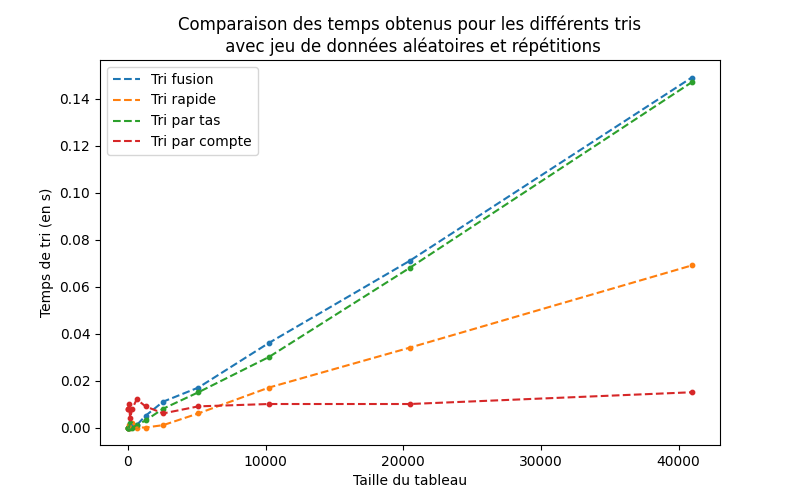
\includegraphics[scale = 0.5]{Images/Courbes img/aléatoire avec rep/aléatoires avec répétitions.png}\\
\underline {Figure 2 – Comparaison des tris pour un jeu de données aléatoires avec redondance}

\subsubsection{Tris sur le jeu de données ordonnées sans redondance}
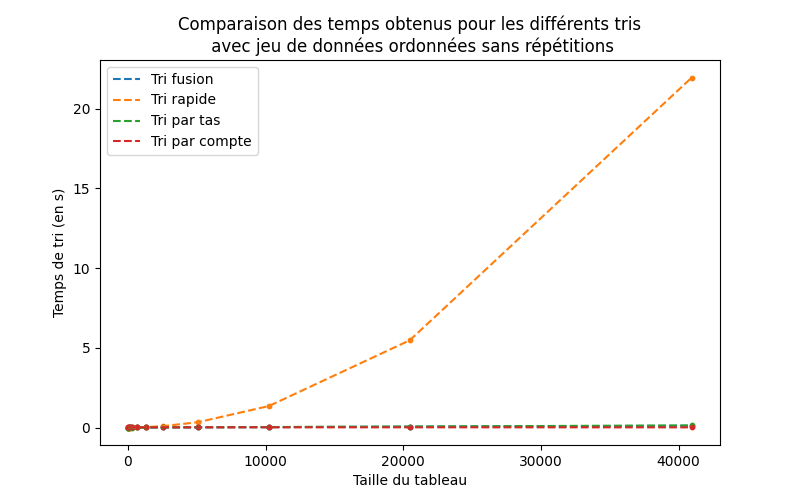
\includegraphics[scale = 0.5]{Images/Courbes img/trié sans rep/ordonnées sans répétitions.png}\\
\underline {Figure 3 – Comparaison des tris pour un jeu de données ordonnées sans redondance}

\subsubsection{Tris sur le jeu de données ordonnées avec redondance}
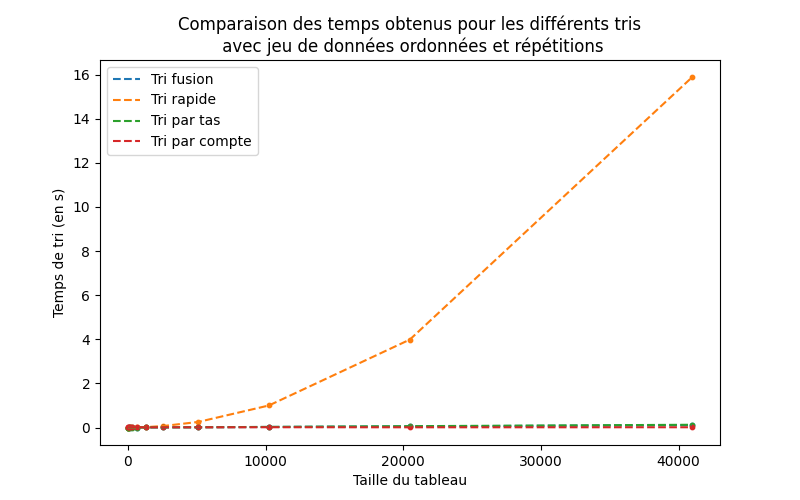
\includegraphics[scale = 0.5]{Images/Courbes img/trié avec rep/ordonnées avec répétitions.png}\\
\underline {Figure 4 – Comparaison des tris pour un jeu de données ordonnées avec redondance}

\subsubsection{Tris sur le jeu de données inversées sans redondance}
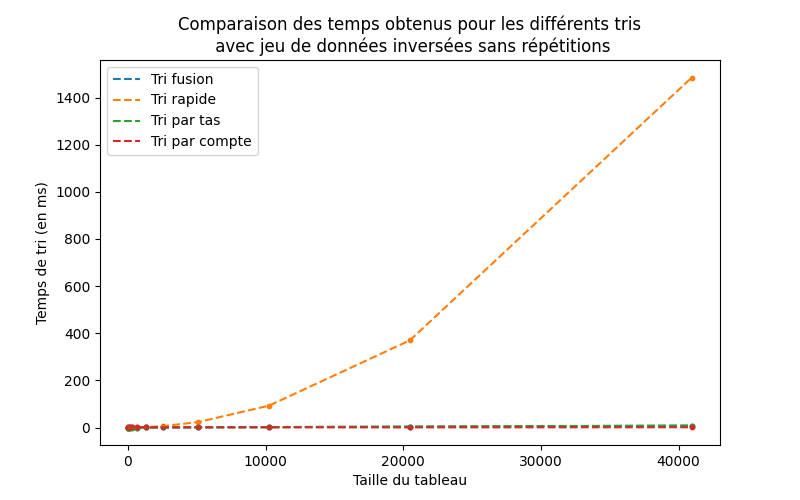
\includegraphics[scale = 0.5]{Images/Courbes img/inversé sans rep/inversées sans répétitions.png}\\
\underline {Figure 5 – Comparaison des tris pour un jeu de données inversées sans redondance}

\subsubsection{Tris sur le jeu de données inversées avec redondance}
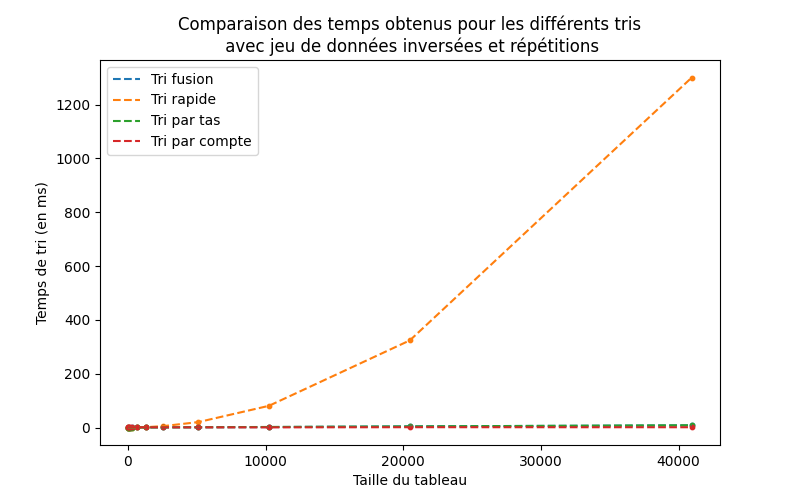
\includegraphics[scale = 0.5]{Images/Courbes img/inversé avec rep/inversées avec répétitions.png}\\
\underline {Figure 6 – Comparaison des tris pour un jeu de données inversées avec redondance}

\vspace{1cm}

On observe donc que quoi qu'il arrive, le tri par comptage reste le plus performant avec une complexité temporelle
quasi linéaire (O($n+k$)) et un temps constament strictement inférieur à 1.2 millisecondes. Viennent ensuite les tris par tas et fusion
qui cotoient la barre des 10 millisecondes dans les cinq cas testés grâce à leur complexité logarithmique $\displaystyle{(O(n * \log{n})}$). Et enfin le tri rapide qui est très efficace sur nos tableaux
remplis aléatoirement est preque deux fois plus rapide $\displaystyle{(O(n * \log{n})}$) mais devient très lent sur des tableaux déja ordonnées et inversés avec une complexité quadratique (O($n^2$)).\\
Pour se donner une idée plus précise des performances de chaque tri sur les différents jeux de données, on peut modifier notre script python et obtenir ceci:\\

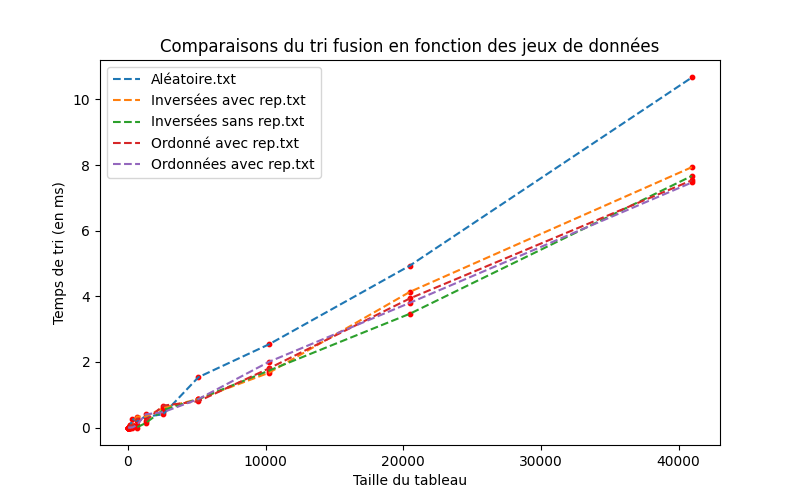
\includegraphics[scale = 0.5]{Images/Courbes img/individuels/tri fusion.png}\\
\underline {Figure 7 – Comparaison des performances du tri fusions sur les cinq jeux de données}

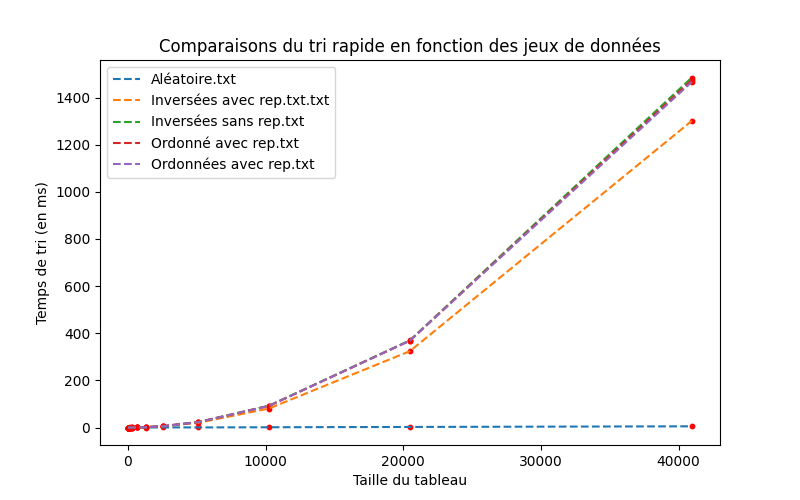
\includegraphics[scale = 0.5]{Images/Courbes img/individuels/tri rapide.png}\\
\underline {Figure 8 – Comparaison des performances du tri rapide sur les cinq jeux de données}

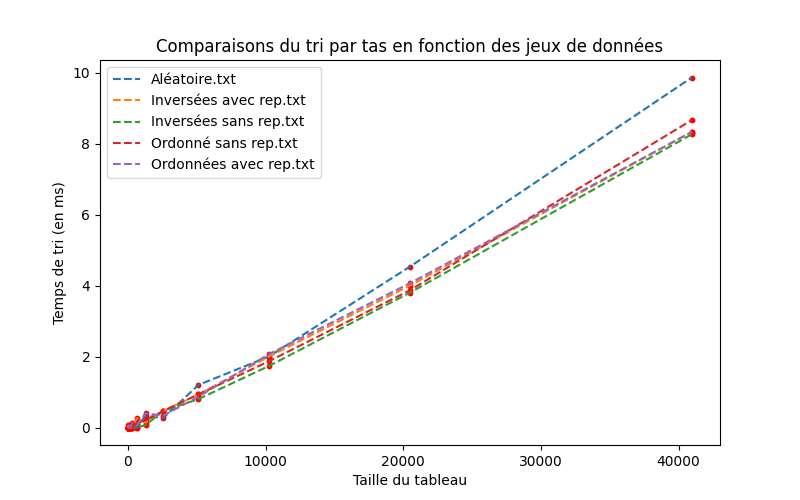
\includegraphics[scale = 0.5]{Images/Courbes img/individuels/tri par tas.png}\\
\underline {Figure 9 – Comparaison des performances du tri par tas sur les cinq jeux de données}

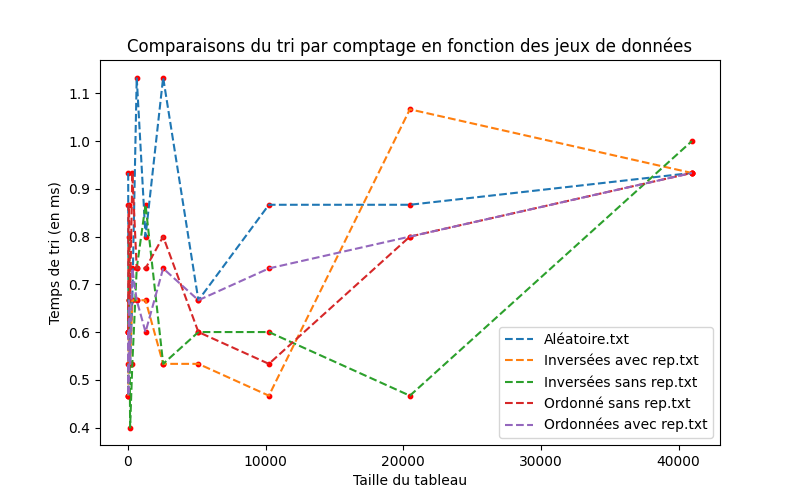
\includegraphics[scale = 0.5]{Images/Courbes img/individuels/tri par comptage.png}\\
\underline {Figure 10 – Comparaison des performances du tri par comptage sur les cinq jeux de données}

\vspace{2cm}

Grâce aux courbes obtenues, on distingue que les tris fusions, par tas et comptage sont tous tois plûtot réguliers quelque soit le type de jeu passé en entrée contrairement au tri rapide.

\section{Limites et algorithmes "hybrides"}
\subsection{L’algorithme de tri parfait}

Après l'étude de ces quelques tris on remarque qu’il n’y a pas d’algorithme qui serait efficace pour tous
les jeux de données. Les tri fusion et tri par tas ont l’avantage d’avoir une complexité
temporelle dans le pire des cas en $\displaystyle{O(n*\log{n})}$ les rendants plus efficaces que le tri rapide sur des
jeux de données ordonnées mais empiriquement le tri rapide est toujours plus efficace sur les autres
jeux (quand il est bien implémenté il peut être deux à trois fois plus rapide que le tri fusion et le
tri par tas). Le tri compte (le seul tri sans comparaisons) est le plus efficace parmi les tris étudiés
mais il peut difficilement être utilisé sur autre chose que des nombres.
Ainsi, il est nécessaire de penser aux inconvénients lorsqu’on choisi un algorithme de tri. Le
tri rapide reste un très bon choix si l’on sait qu’on a très peu de chances de tomber sur des jeux
de données ordonnées. David Musser a cependant su pallier au défaut du tri rapide (sa complexité
dans le pire des cas en $\displaystyle{O(n^2))}$ en inventant l’introspective sort.

\subsection{L’introspective sort}
L’introspective sort est un algorithme de tri "hybride", son principe est assez simple : utiliser un compteur de récursivité.
Lorsque la profondeur de récursion dépasse $\displaystyle{K * \log{(n)}}$ (avec K une
constante) on tri le sous-tableau restant avec un algorithme dont la complexité est $\displaystyle{O(n\log{(n)}}$
dans tous les cas (tri par tas, tri fusion, ...).

\section{Conclusion}
Les tris compte, rapide, fusion et par tas sont très performants bien qu’ils présentent des
inconvénients. Mais c’est en combinant de la bonne façon ces algorithmes que l’on conçoit des
algorithmes encore plus efficaces (bien que plus complexes) qui peuvent être utilisés avec de très
grosses données. Dans ce cas-là même les tris moins rapides (comme le tri par insertion) peuvent
être utiles.

\end{document}